
\subsection{Comparing Different Kinds of Cycles}

%  A level is an integer between $1$ and $L$. Level $1$ will be called the finest level, and level $L$ will be called the coarsest level. In the multi-grid algorithm, we
%  consider computations at every different level in a determined order. 
In this Section we compare different types of cycles and study how the number of \textit{Relaxation} steps influence MG's convergence.
MG's cycles start and end on the finest grained grid and are defined by the order in which its different coarseness levels are applied.
The simplest cycle is the V-cycle, already described in Section~\ref{sec:intro}, where a few iterations
  of an iterative method (the \textit{Relaxation} step) is performed at each level from the finest to the coarsest level and then in the reverse order. 
Another common approach is the W-cycle scheme where the coarsest grid level is reached twice before going back to the finest grid level.
It is possible to generalize the notion of cycle to a $k$-cycle (where a V-cycle is a $1$-cycle and a W-cycle is a $2$-cycle).
Figure~\ref{fig.cycles} shows a representation of the V- and the W-cyles with 4 levels where we can see how the W-scheme goes back and forth the coarsest level 4 times before reaching again the finest level of the grid.

%In this context, the MG algorithm makes use of many different input parameters 
% such as the iterative method used, the type of cycle and its number of repetitions, the number of \textit{Relaxation} at each level or the number of different levels to define.
%In this subsection we focus on comparing different types of cycles and study how the number of \textit{Relaxation} steps influence the convergence of the algorithm.
  
%We consider 2 types of cycles: the V-cycle and the W-cycle. 
%The main difference between them is that in the W-cycle the recursive call
%to a coarser grid is made twice instead of one before going back to a finer level. 
%We call these cycles V-cycle and W-cycle because of how we can draw them if we represent each time relaxations are done
%  at a level by a point (see Figure~\ref{fig.cycles}). 
%Figure~\ref{fig.cycles} shows a representation of the V- and the W-cyles.
%It is possible to define other types of cycles by adding more and more repeats of these steps (do $k$ times those steps) to generalize
%  the notion of cycle to a $k$-cycle (where a V-cycle is a $1$-cycle and a W-cycle is a $2$-cycle).
  
 \begin{figure}
 \resizebox{\linewidth}{!}{
 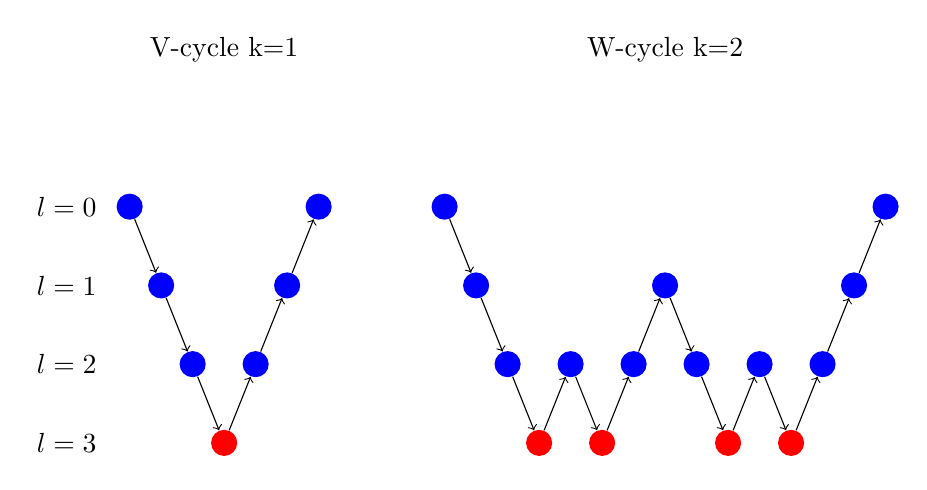
\begin{tikzpicture}
  
\begin{scope}[xscale=2/5]

  \node (sh) at (-5,3) { $l=0$ };
  \node (shh) at (-5,2) { $l=1$ };
  \node (shhh) at (-5,1) { $l=2$ };
  \node (shhhh) at (-5,0) { $l=3$};
  
  \node (title) at (0,5) { V-cycle k=1};
  \node (title2) at (14,5) {W-cycle k=2};

    \node[circle,fill=blue] (a) at (-3,3) { };
    \node[circle,fill=blue] (b) at (-2,2) {};
    \node[circle,fill=blue] (c) at (-1,1) {};
    \node[circle,fill=red] (d) at (0,0) {};
    \node[circle,fill=blue] (e) at (1,1) {};
    \node[circle,fill=blue] (f) at (2,2) {};
    \node[circle,fill=blue] (g) at (3,3) {};
    
    \draw[->] (a) -- (b);
    \draw[->] (b) -- (c);
    \draw[->] (c) -- (d);
    \draw[->] (d) -- (e);
    \draw[->] (e) -- (f);
    \draw[->] (f) -- (g);
    
    \node[circle,fill=blue] (aa) at (7,3) { };
    \node[circle,fill=blue] (ab) at (8,2) {};
    \node[circle,fill=blue] (ac) at (9,1) {};
    \node[circle,fill=red] (ad) at (10,0) {};
    \node[circle,fill=blue] (ae) at (11,1) {};
    \node[circle,fill=red] (af) at (12,0) {};
    \node[circle,fill=blue] (ag) at (13,1) {};
    \node[circle,fill=blue] (ah) at (14,2) {};
    \node[circle,fill=blue] (ai) at (15,1) {};
    \node[circle,fill=red] (aj) at (16,0) {};
    \node[circle,fill=blue] (ak) at (17,1) {};
    \node[circle,fill=red] (al) at (18,0) {};
    \node[circle,fill=blue] (am) at (19,1) {};
    \node[circle,fill=blue] (an) at (20,2) {};
    \node[circle,fill=blue] (ao) at (21,3) {};
    
    \draw[->] (aa) -- (ab);
    \draw[->] (ab) -- (ac);
    \draw[->] (ac) -- (ad);
    \draw[->] (ad) -- (ae);
    \draw[->] (ae) -- (af);
    \draw[->] (af) -- (ag);
    \draw[->] (ag) -- (ah);
    \draw[->] (ah) -- (ai);
    \draw[->] (ai) -- (aj);
    \draw[->] (aj) -- (ak);
    \draw[->] (ak) -- (al);
    \draw[->] (al) -- (am);
    \draw[->] (am) -- (an);
    \draw[->] (an) -- (ao);
    \end{scope}
    
 \end{tikzpicture}}
 \caption{V-cycle and W-cycle on 4-level grid.}
 \label{fig.cycles}
\end{figure}

\begin{table}

\begin{center}
 \begin{tabular}{|c|c|c|c|c|c|c|c|c|}
   \hline
   Type of cycle & V & V & V & V & W & W & W & W \\
   \hline
   $\alpha$ & 1 & 2 & 3 & 10 & 1 & 2 & 3 & 10 \\
   \hline
 \end{tabular}
\end{center}
 \caption{8 strategies.}
 \label{table.strat1}

\end{table}


\begin{figure*}
  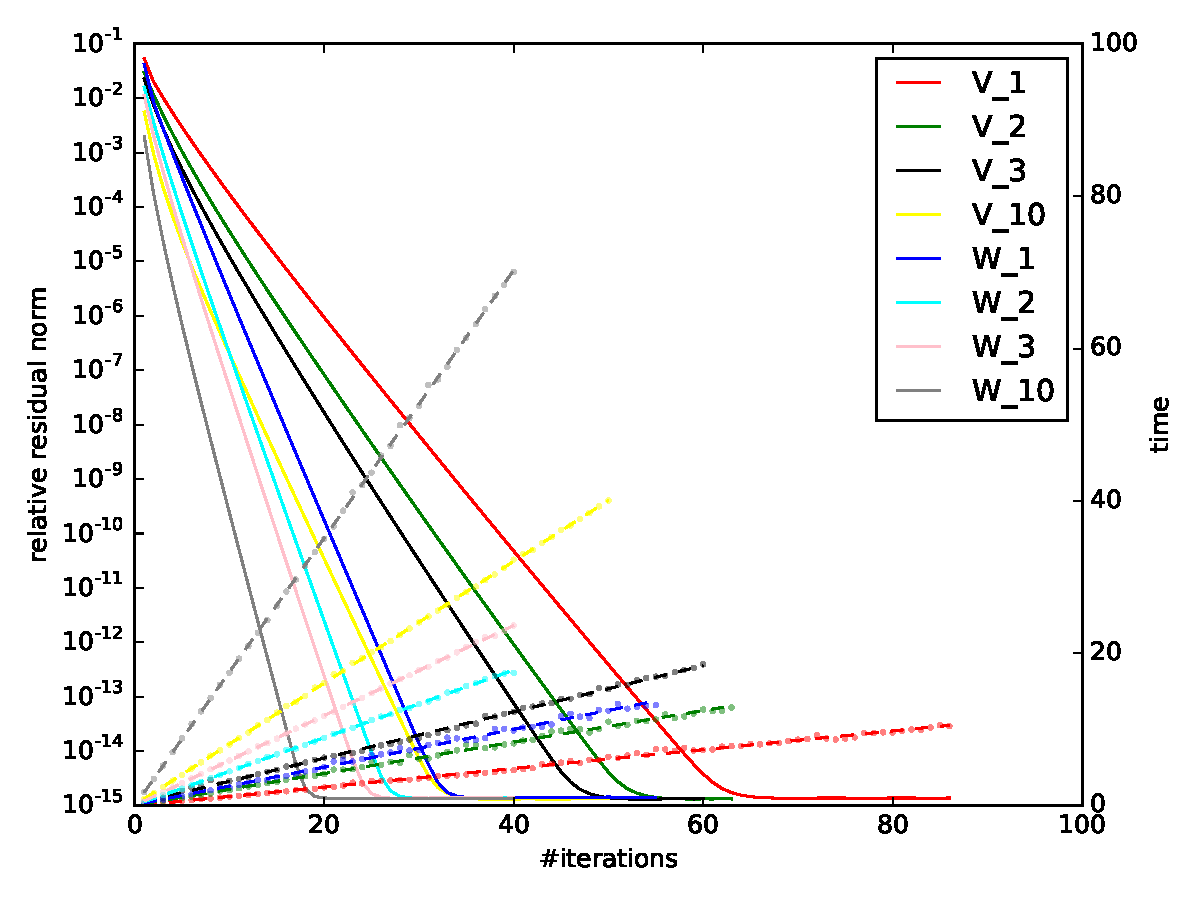
\includegraphics[width=0.49\linewidth]{figs/convergence_1.pdf}
  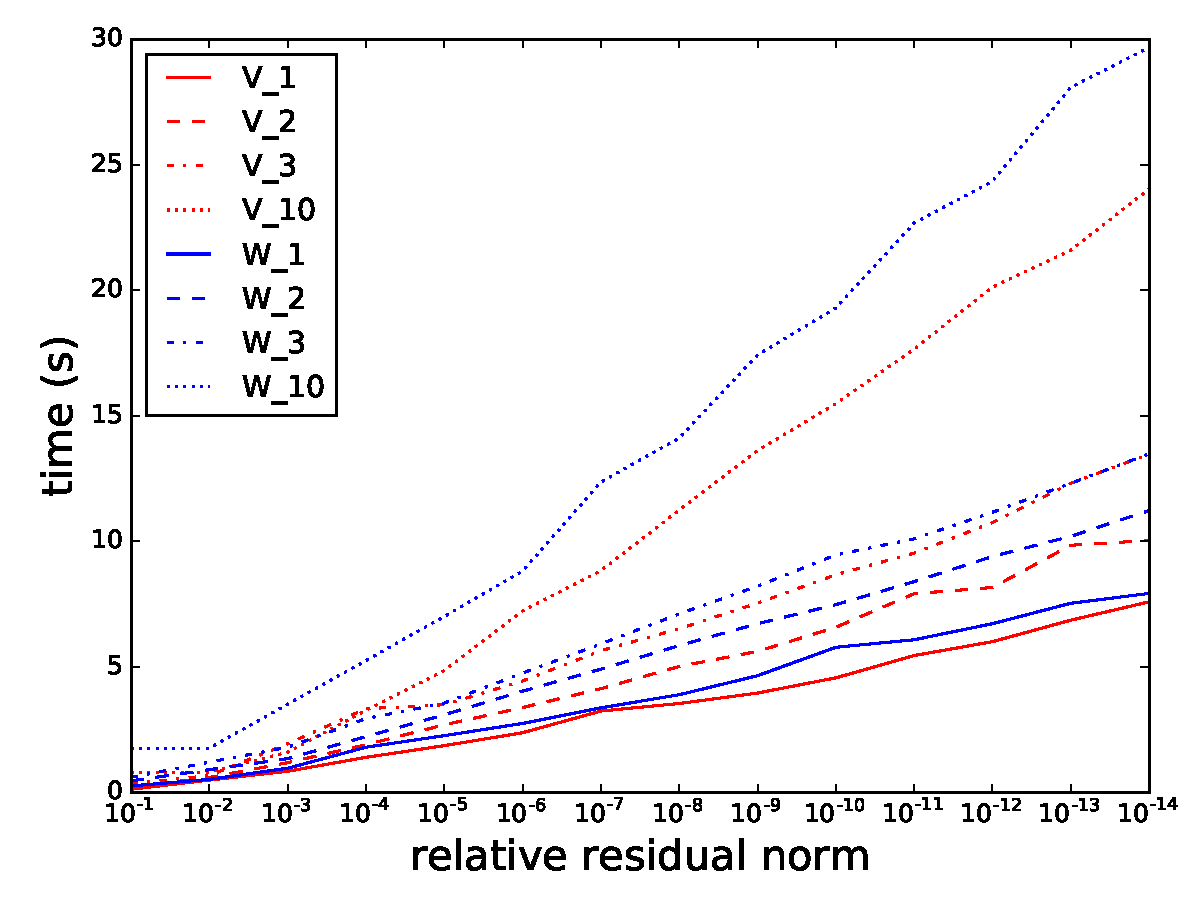
\includegraphics[width=0.49\linewidth]{figs/time_convergence.pdf}
  \caption{Execution time and final residual norm of the 8 strategies per iteration (left) and convergence time as a function of the tolerance (right).}
  \label{fig.first_tests}
\end{figure*}


The MG algorithm makes use of many different input parameters that have an impact on its success. 
% such as the iterative method used, the type of cycle and its number of repetitions, the number of \textit{Relaxation} steps per level or the number of different levels to define.
In our context, we define a strategy as a combination of values of the most relevant parameters: The type of cycle (V or W), the number of relaxation steps $\alpha$, and the total number of coarseness levels of the grid. 
%The default implementation of BomerAMG does not allow to have different values
%for $\alpha_1,\alpha_2,\dots$ so we set them all to this value $\alpha$. 
We consider a total of 8 different strategies represented in Table~\ref{table.strat1} where we consider V- and W-cycles and we perform 1, 2, 3 and 10 relaxation steps for eack kind of cycles, having a total of 8 configurations. 
The number of different coarseness levels of the grid is 8.
To compare the different strategies we consider an input matrix of size $512000 \times 512000$, 
and a maximum number of cycles from 1 to 100.
The algorithm's tolerance is set to $0$ to always reach the maximum number of cycles (1 to 100 depending on the experiments).
We measure for each experiment the final relative residual norm and the execution time. 
Each experiment is run 10 times to have an accurate average execution time.

The results are presented on Figure~\ref{fig.first_tests}.
The left figure shows how the accuracy evolve with the number of cycles performed (plain lines) while also showing the total execution time (dashed lines). For example, we see that the V cycle with 1 relaxation step (in red) is less costly in term of execution time but converges with more cycles than the other strategies. To be able compare the convergence speed, we present the cost of reaching
a given accuracy on the right figure (left of the x-axis is a small tolerance i.e. correspond to accurate results while the right of the x-axis represent inaccurate (but fast) results).
What we can observe is that, as expected, increasing the number of relaxation steps or complexifying the cycle increases the overall time to do one cycle. However, it converges in less iterations.
We see on the right figure that actually, for a given precision, the simple V-cycle with only 1 relaxation at each step is the fastest way to reach it, followed closely by the W-cycle with $\alpha=1$.\\
The conclusion is that relaxation steps seem to be too costly for the accuracy they grant. It is better to increase the complexity of the cycle or do more cycles, thus more moves in the grid, than doing more relaxation steps. This at least proves
that multi-grid is a good alternative to classic iterative methods.
